%% ---------------------------------------------------------------------
%% Copyright 2014, Thales, IGN, Rémi Cura
%% 
%% This file contains the introduction of article
%% ---------------------------------------------------------------------


\section{Introduction}

\begin{figure*}[t!]
	\begin{center}
		\fbox{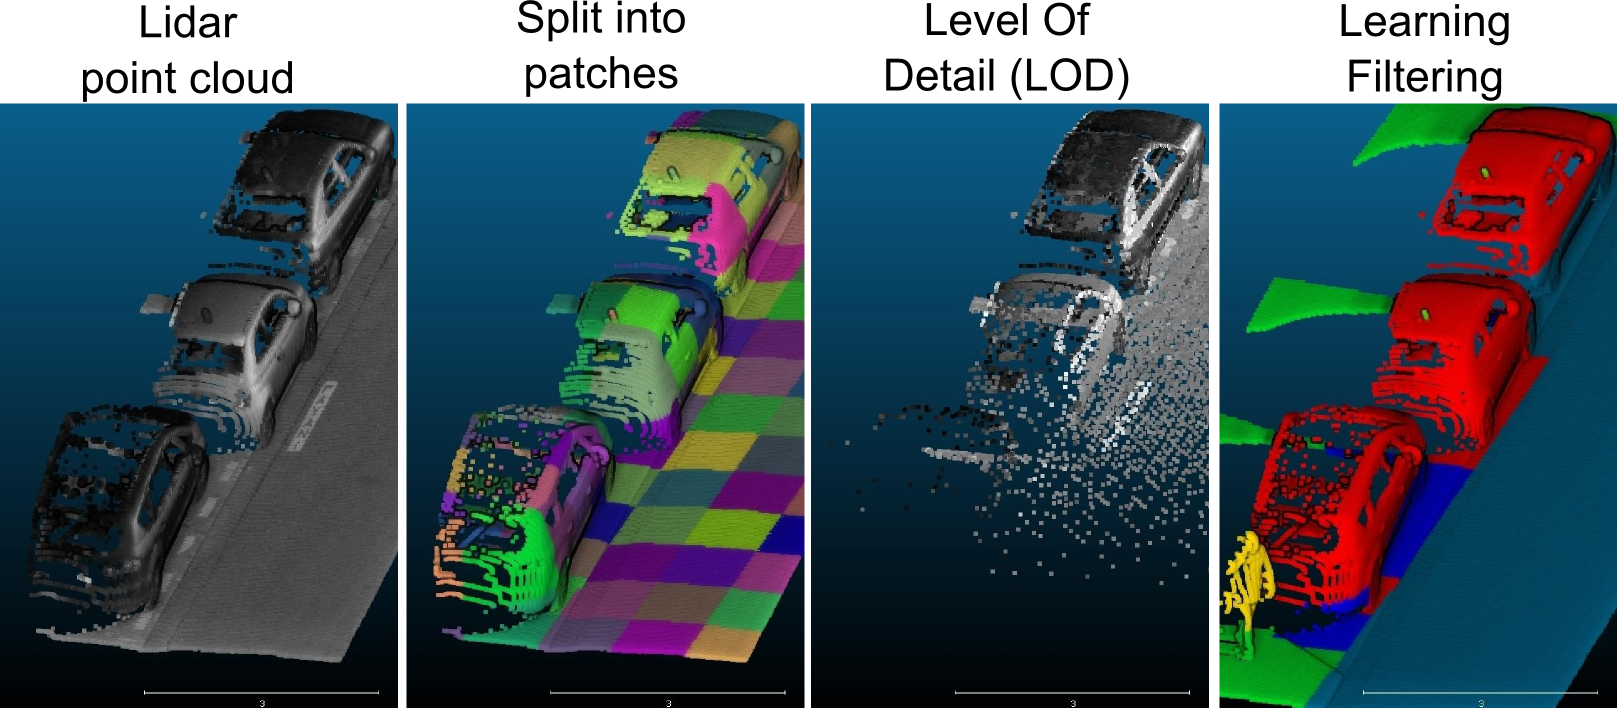
\includegraphics[width=\textwidth,keepaspectratio ]{./illustrations/chap2/banner_for_paper.png}}
		\caption{Graphical Abstract : a Lidar point cloud (1), is split it into patches (2) 
		and stored in the PCS (\cite{Cura2015}), patches are re-ordered to obtain free LOD 
		(3 : a gradient of LOD here).
		Lastly the ordering is used as a feature for learning and efficient filtering (4) } 
		\label{lod.fig:banner_image}
	\end{center}
\end{figure*} 

	\subsection{Problem}  
		Point cloud data is becoming more and more common. Following the same trend, the acquisition frequency and precision of the Lidar device are also increasing.
		Thus point cloud processing is entering in the Big Data realm.
		Point cloud data usage is also spreading and going out of their traditional user communities. 
		Lidar are now commonly used by non-specialized users. 
		The now common datasets in the multi billion point range can not fit in computer memory. 
		Furthermore, having the complete and fully detailed point cloud is impracticable, unnecessary, or even damageable for most applications.
		
		Reducing the number of point is then a vital need for practical point cloud management.
		
		There are basically two levers to reduce the amount of data considered. The first would be \textbf{filtering} data based on characteristics (position, time, semantic, etc.), thus keeping the original data, but only a portion of it.
		The second lever would be to generalise the data, that is replace many points with few objects that represent them well. Those objects can be more abstract (geometric primitives like plane for example), or simply some well chosen points (subset).
		
		For instance, to visualize the parts of a massive point cloud, we might fetch only the points that are visible (filtering),
		and not display all the points but only the sufficient number to understand the scene (generalisation).
		(See Figure \ref{lod.fig:two_reduction})
		\myimage{"./illustrations/chap2/two_reduction_strategy/two_reduction_strategy"}{Two strategies to limit the amount of points to work on.}{lod.fig:two_reduction}
		
		The system we propose un \cite{cura2015} is compatible with both, and extensively covers the filtering and abstracting part. In this article we focus on the generalisation problem using points.
		
		Thus we deal with a simpler version of a problem common for Geographical Information System (GIS): how to generalize information contained in huge datasets, that is reduce the details of the data while retaining its principal organisation.
		 
		This problematic is very commons accross research field, and could be seen as a problem of compression, clustering, dimensionality reduction, etc.
	  
		This particular problem applied to visualisation is commonly called Level Of Details (LOD, cf \href{lod.banner_image}{figure ~\ref{lod.fig:banner_image}}).
		
		The problem is then how to reduce the amount of points while preserving the geometric characteristics of the underlying sensed object, in an efficient manner, and while being robust to the way the sensing was done?
		Indeed LOD approaches sacrifices of a part of information in exchange of a massive reduction of data size which is necessary for efficient usage/visualisation. In this regard, a LOD method must by nature be efficient, or the information loss would be pointless.
		
		

	\subsection{Related Work} 
		
        \todoall{ajouter citation de bereuter \protect\cite{Bereuter2015} , \protect\cite{Schwartges2013} \protect\cite{sester2001}  }
        
        \todoall{parler de Latin Hypercube sampling : c est le nom savant poru faire une grille 3D et prendre un echantillon max par voxel}
        
        \todoall{parler de Rainville2012, un bon résumé de ce qui se fait}
        
        \todoall{parler de Halton sequence, low discrepancy comme autre candidats à sampler uniformément l espace avec un peu d'aléatoire}
        
        \todoall{parler de l'alternative : reconstruire une surface, interpoller les attributes dessus, puis choisir le point centrale --> depend de la présence d'une surface; 
        ou methode d'optimisation, comment construire le point qui minimiserait l erreur}
    
	    \todoall{construction de quadtree a partir de Z curve? "Index and Query Methods in Road Networks"}
	    
	    \todoall{regarder https://octomap.github.io/}
	    
	 
        Fil rouge à raconter : on veut en fait sampler les fonctions x,y,z, attributs.
        Ce dont on est sur c est x,y,z, donc dans l ideal on trouverait le sampling sur la surface qui minimise la perte d erreur. Comme on est meme pas sur d avoir une surface, on peut pas faire ça. On a meme pas un sampling uniforme, ce qui nous interdit d utiliser les moindres carrées (pas le choix, c est la variation de densité qui le veut).
        A la place on prend l autre approche, on crée un sampling regulier, et comme on veut pas se dépatouiller des attributs, on prend un point déjà existant.
        De plus on veut pouvoir etre utile az plusieurs applciations, donc on cherche pas le meilleur lod pour une application, mais un bon lod pour toutes les applications.
       
        
        Because points are not only 3D but may also have attributes, a perfect ordering would require extensive knowledge of those attributes and of the usage to be made with the point cloud.
        For instance lets consider a point cloud containing a classification, and suppose the application is to identify the presence of a very rarely present class C.
        In this case a purely geometrical LOD would probably hide C until the very detailed levels, as such the optimal ordering strategy would need to depend on this classification attributes.
        Orthogonally, even when using only the geometry to order points, the ordering may again depend on the application. For instance an application of visualisation of point cloud of man-made objects would probably benefits from ordering points based on curvature (as an approximation of visual saliency).
        
        
        
        \todoall{parler de \cite{Trapp2008} en precisant que visualisation et generalisation peuvent etre mélangé, et que ce n'est pas toujours une question de perfomance, mais de choisir ce que l'utilisateur voit (similaire au flou au cinéma)}
		One way to tackle data size is to use a Level Of Detail strategy. Octree methods have been common in computer graphics for several decades \citep{Meagher1982}. They are used in many methods to speed computing, or compress data, like in the work of \cite{Schnabel2006,Huang2006} (which have not been designed to scale).
		
		
		We can see point cloud as a sampling of a surface (or volume) of the sensed object. This sensing may be structured for the sensing device (for instance a Lidar may sense point using a constant angle), but not necessary for the sensed object (see figure \ref{lod.fig:irregular_sampling})
		\myimage{"./illustrations/chap2/problem_in_sampling/regular_vs_irregular_sampling"}{Regular sensing does not imply regular sampling.}{lod.fig:irregular_sampling}.
		
		\cite{Elseberg2013} give a good overview of octree usage for point clouds. Their method proposes to directly store the points and octree in a file. They explore many applications that could benefit from our method (visual LOD, registration, processing). We share many objectives. It is an extremely effective approach that also enables visual LOD, but is very specialized on geometry. In particular, this method is not integrated with other GIS data (Geographical Information System), point cloud fast querying is not possible on attributes or metadata, and point cloud format is extremely specific.
		\\
		Another orthogonal way is to not use file, but store point cloud in DBMS.  \cite{vanOosterom2014} implements such system at very big scale and discuss how it can answer to various need. This approach has gained recent interest (\cite{pgPointCloud2014}) because it is generic, it scales naturally to very large data set and is easier to implement than starting from scratch. We also observe that most of Big Data system use methods from the DBMS world.
		\\ 
		\cite{Demantke2014} introduces a sophisticated per-point dimensionality descriptor, which is used to find optimal neighbourhood size. A main difference is that this feature is computed for each point (thus is extremely costly to compute), and that dimensionality is influenced by density variation.
		
		Random Forest method started with \cite{Amit97shapequantization} and theorized by \cite{Breiman2001} and has been very popular since then. They are for instance used by \cite{Golovinskiy2009} who perform object detection, segmentation and classification. They analyse separately each task on an urban data set, thus providing valuable comparison. Their method is uniquely dedicated to this task, like \cite{Serna2014} who provide another method and a state of the art of the segmentation/classification subject.
		Both of this methods are in fact 2D methods, working on an elevation image obtained by projecting the point cloud. However we observe that street point clouds are dominated by vertical surfaces, like building (about 70\% in Paris data set). Our method is fully 3D and can then easily be used to detect vertical object details, like windows or doors on buildings.
		 
	
	\subsection{Contribution}
		This paper re-uses and combines existing and well established methods with a focus on simplicity and efficiency. As such, all the methods are tested on billions scale point cloud, and are Open Source for sake of reproducibility test and improvements.
		We propose a simple method that enables portable, computation-free, geometrical Level Of Detail.
		Our first contribution is to propose to store the LOD information directly into the ordering of points rather than externally, avoiding any data duplication.
		Thus, we don't duplicate information, and the more we read points, the more precise of an approximation of the point cloud we get. If we read all the points, we have the original point cloud.
		
		The second contribution is a simple way to order points in order to have an increasingly better geometric approximation of the point cloud when following this order.
		
		The third contribution is to show that this ordering embed information about the dimensionality of the sensed object,
		to the point of being a simple and free dimensionality descriptor.
		We demonstrate the interest of this descriptor by performing a Random Forest classification that can then be used for very fast pre-filtering of points, and other applications.
			
		
	\subsection{Plan of the article}
		The rest of this article is organized as follows:
		in the next section \ref{lod.sec:method} we present the methods.  
		In the result section \ref{lod.sec:result} we give the results.
		We discuss it and the possible limitations in section \ref{lod.sec:discussion}.
		
		Following the IMRAD format~\citep{Wu2011}, the remainder of this article is divided into three sections.
		Section~\ref{lod.sec:method} presents the LOD solution, how it produces a dimensionality descriptor, and how this can leveraged for classification.  
		Section~\ref{lod.sec:result} reports on the experiments validating the methods.
		Finally, the details, the limitations, and potential applications are discussed in Section~\ref{lod.sec:discussion}.
		
